% !TeX root = ..\..\main.tex
\section{ARMA and ARIMA Model}

The first step in building an autoregressive (integrated) moving average (AR(I)MA) model is to determine which process best describes our data. Our process is considered to consist of:

\begin{multicols}{3}
    Autoregressive:
    \begin{equation*}
        \AR{p}: x_t = \sum_{i=1}^p\alpha_ix_{t-i} + \epsilon_t
    \end{equation*}
    \vfill
    \columnbreak
    \noindent Integrated: d is the degree of differencing (the number of times the data have had past values subtracted).
    \vfill
    \columnbreak
    Moving Average:
    \begin{equation*}
        \MA{q}: x_t = \sum_{i=0}^q\beta_i\epsilon_{t-i}
    \end{equation*}
    \vfill
    \columnbreak
\end{multicols}

Where $x_t$ represents the value measured at the $t^{\text{th}}$ time step ($\Delta t$) and $\epsilon_t$ are identical and independent realizations from a normal (Gaussian) distribution with zero mean and variance $\sigma^2$. 

\subsection{Autoregressive Moving Average Model (ARMA)}

An ARMA model only consist off the $\AR{p}$ and $\MA{q}$ often referred to as $\ARMA{p}{q}$ but is identical to \break$\ARIMA{p}{0}{q}$, expressed mathematically as:

\begin{equation*}
   \ARMA{p}{q} : x_t  = \sum_{i=1}^p\alpha_ix_{t-i} + \sum_{i=0}^q\beta_i\epsilon_{t-i} \quad \text{where } \epsilon_t \sim \text{N}\left(0, \sigma^2\right)
\end{equation*}

Our problem then is to fit parameters $(p,q)$ that best describe the underlying process of data.

\subsubsection{Finding optimal parameters}\label{SSec:fop1}

It is possible that our data may have one of the parameters equal 0 meaning that we just an AR or MA process. One way to check this is to calculate both the auto correlation (ACF) and partial auto correlation functions (PACF). Then using the table below we can see if our data satisfies the criteria.
\par\medskip
\begin{center}
    \begin{tabular}{c|c|c|c}
        & AR(p) & MA(q) & ARMA(p,q) \\
        \hline ACF & Tails off & Cuts off after lag $q$ & Tails off \\
        PACF & Cuts off after lag $p$ & Tails off & Tails off \\
    \end{tabular}
\end{center}
\par\medskip
The ACF and PACF functions of our data is shown in \autoref{S2fig:ACFPACF}. Taking a look at the ACF \autoref{S2fig:ACF} we see that we have two peaks at 0.25 and 1.00 (excluding peak at 0). Then looking at the PACF \autoref{S2fig:PACF} we have one peak at 0.75 but also one peak just below the 95\% confidence interval at 0.25. Since any of these peaks could be down to noise, it is hard to exactly determine our parameters from this analysis alone.

\begin{figure}[H]
    \centering
    \begin{subfigure}[b]{\sOneSize\textwidth}
        \centering
        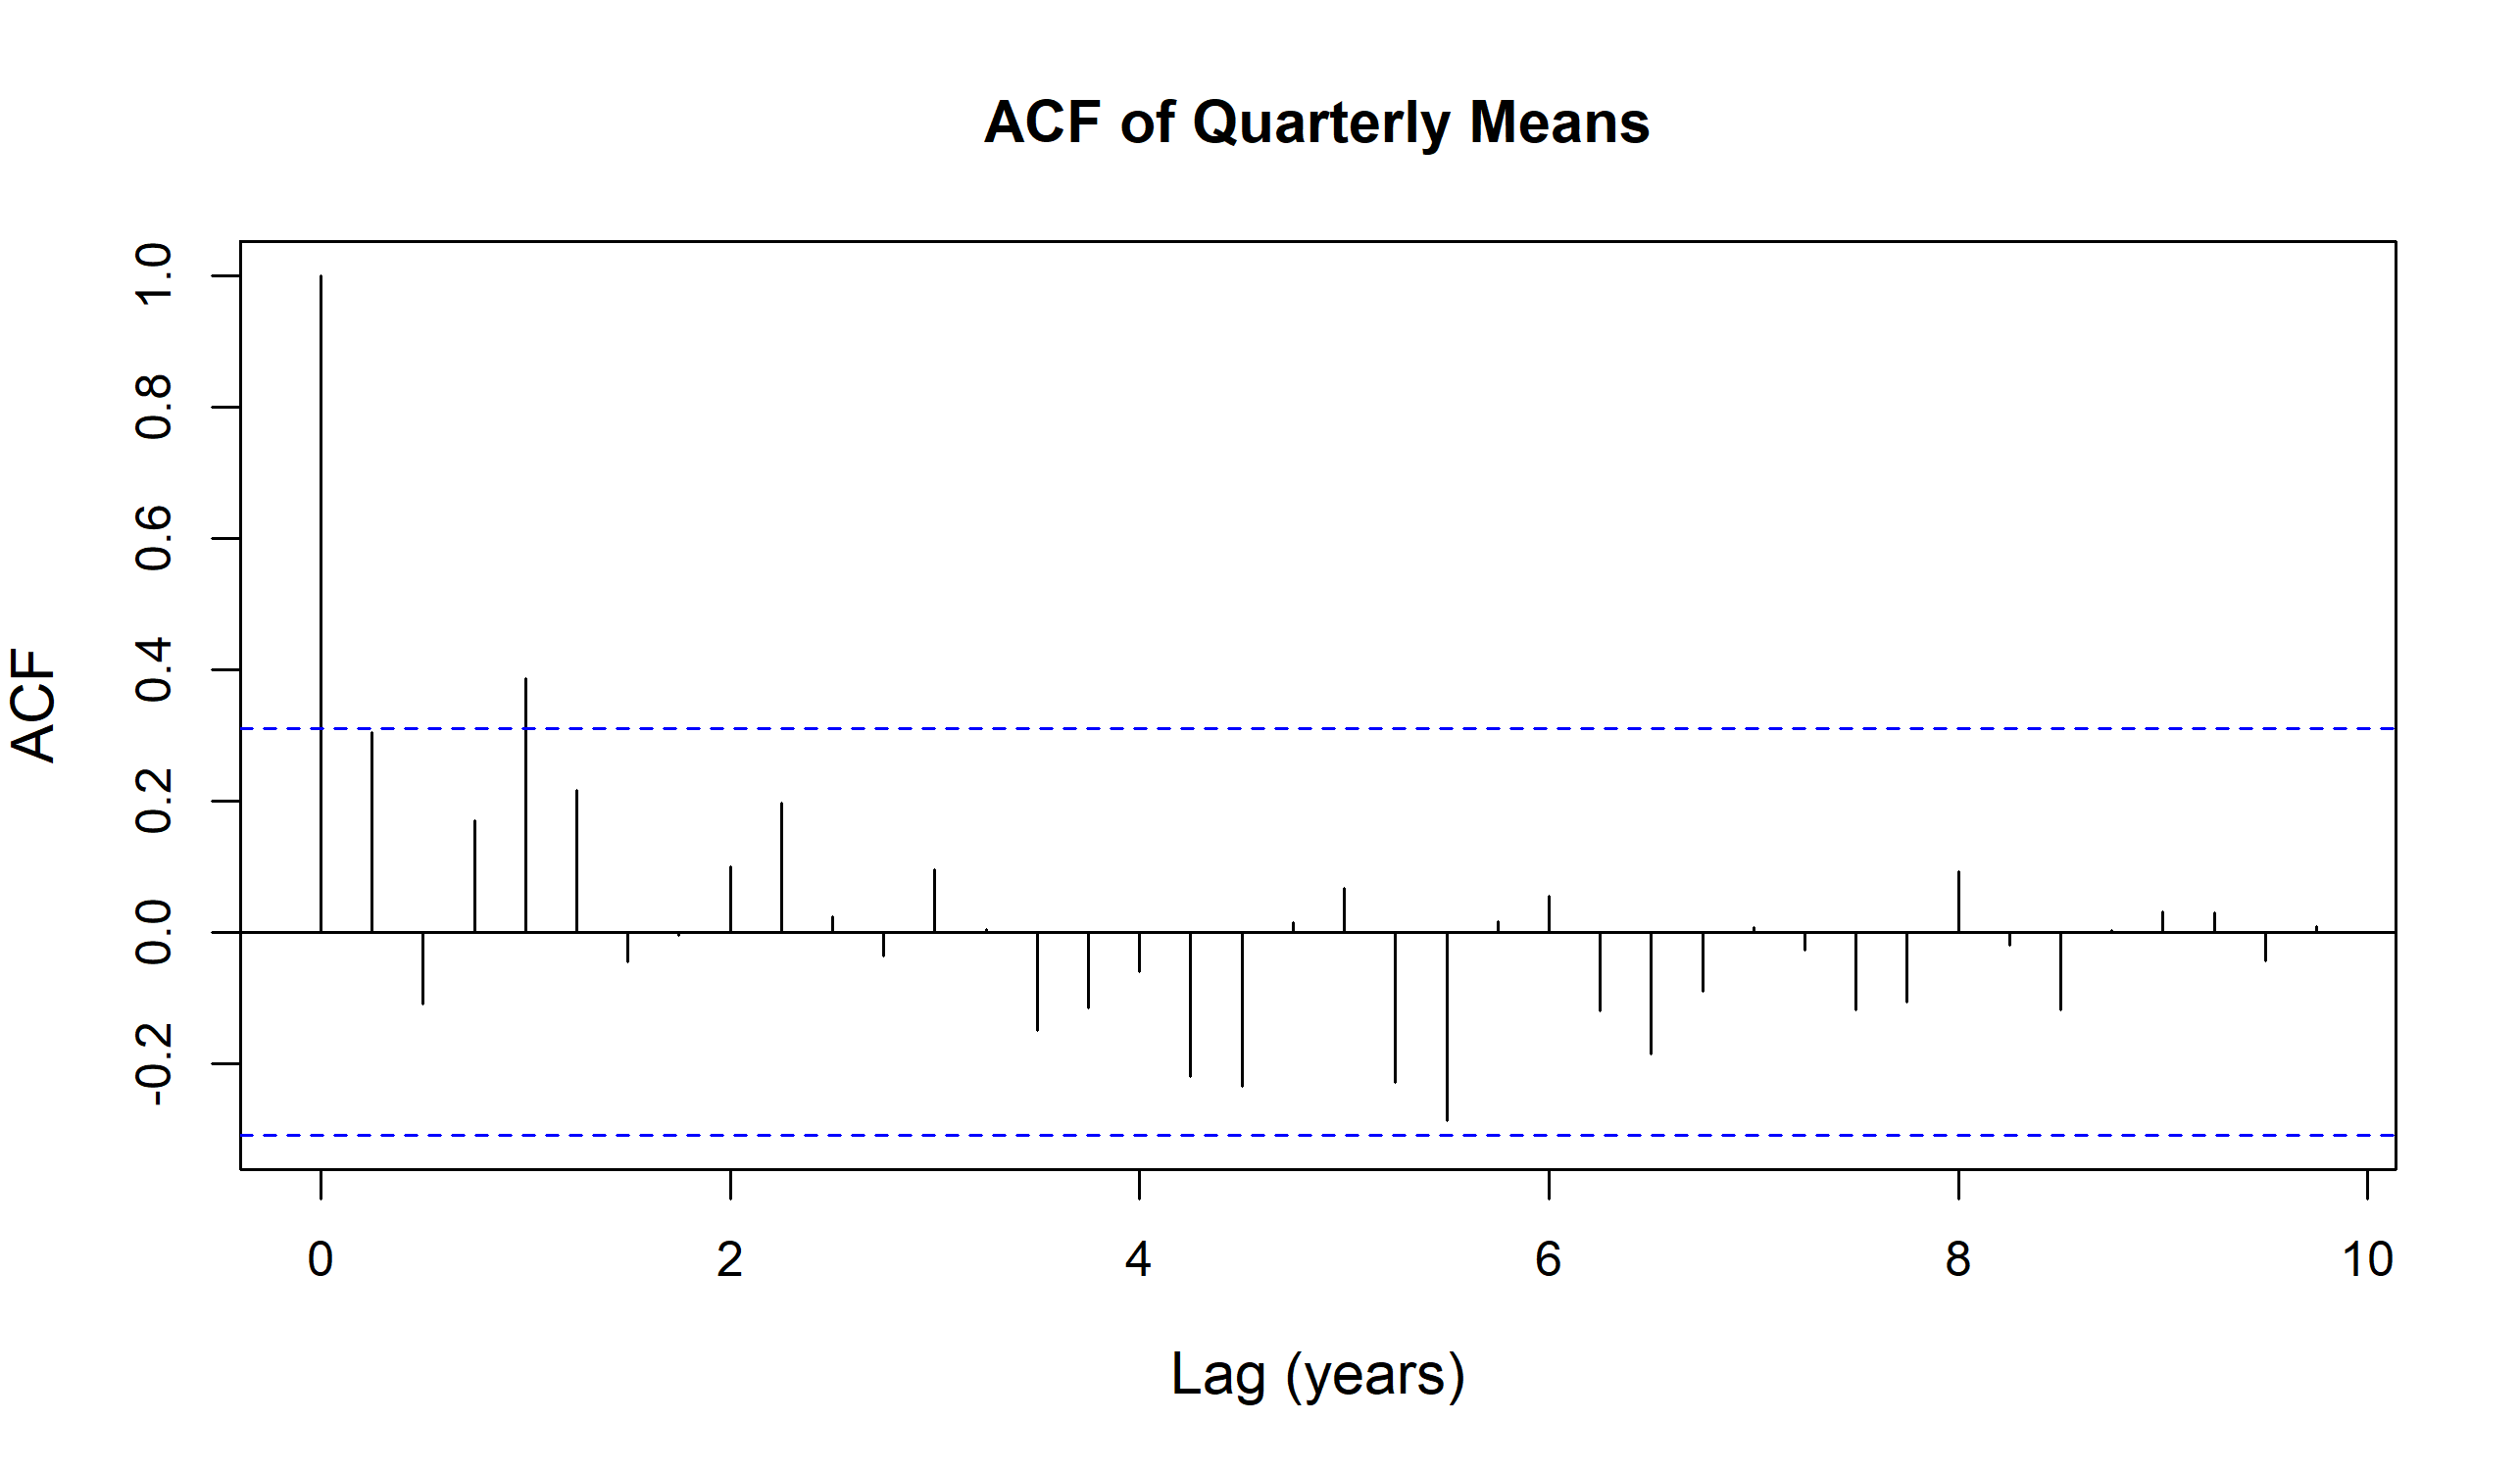
\includegraphics[width=\textwidth]{Sections/ARIMA/Plots/ACF.png}
        \subcaption{Auto correlation function}\label{S2fig:ACF}
    \end{subfigure}
    \begin{subfigure}[b]{\sOneSize\textwidth}
        \centering
        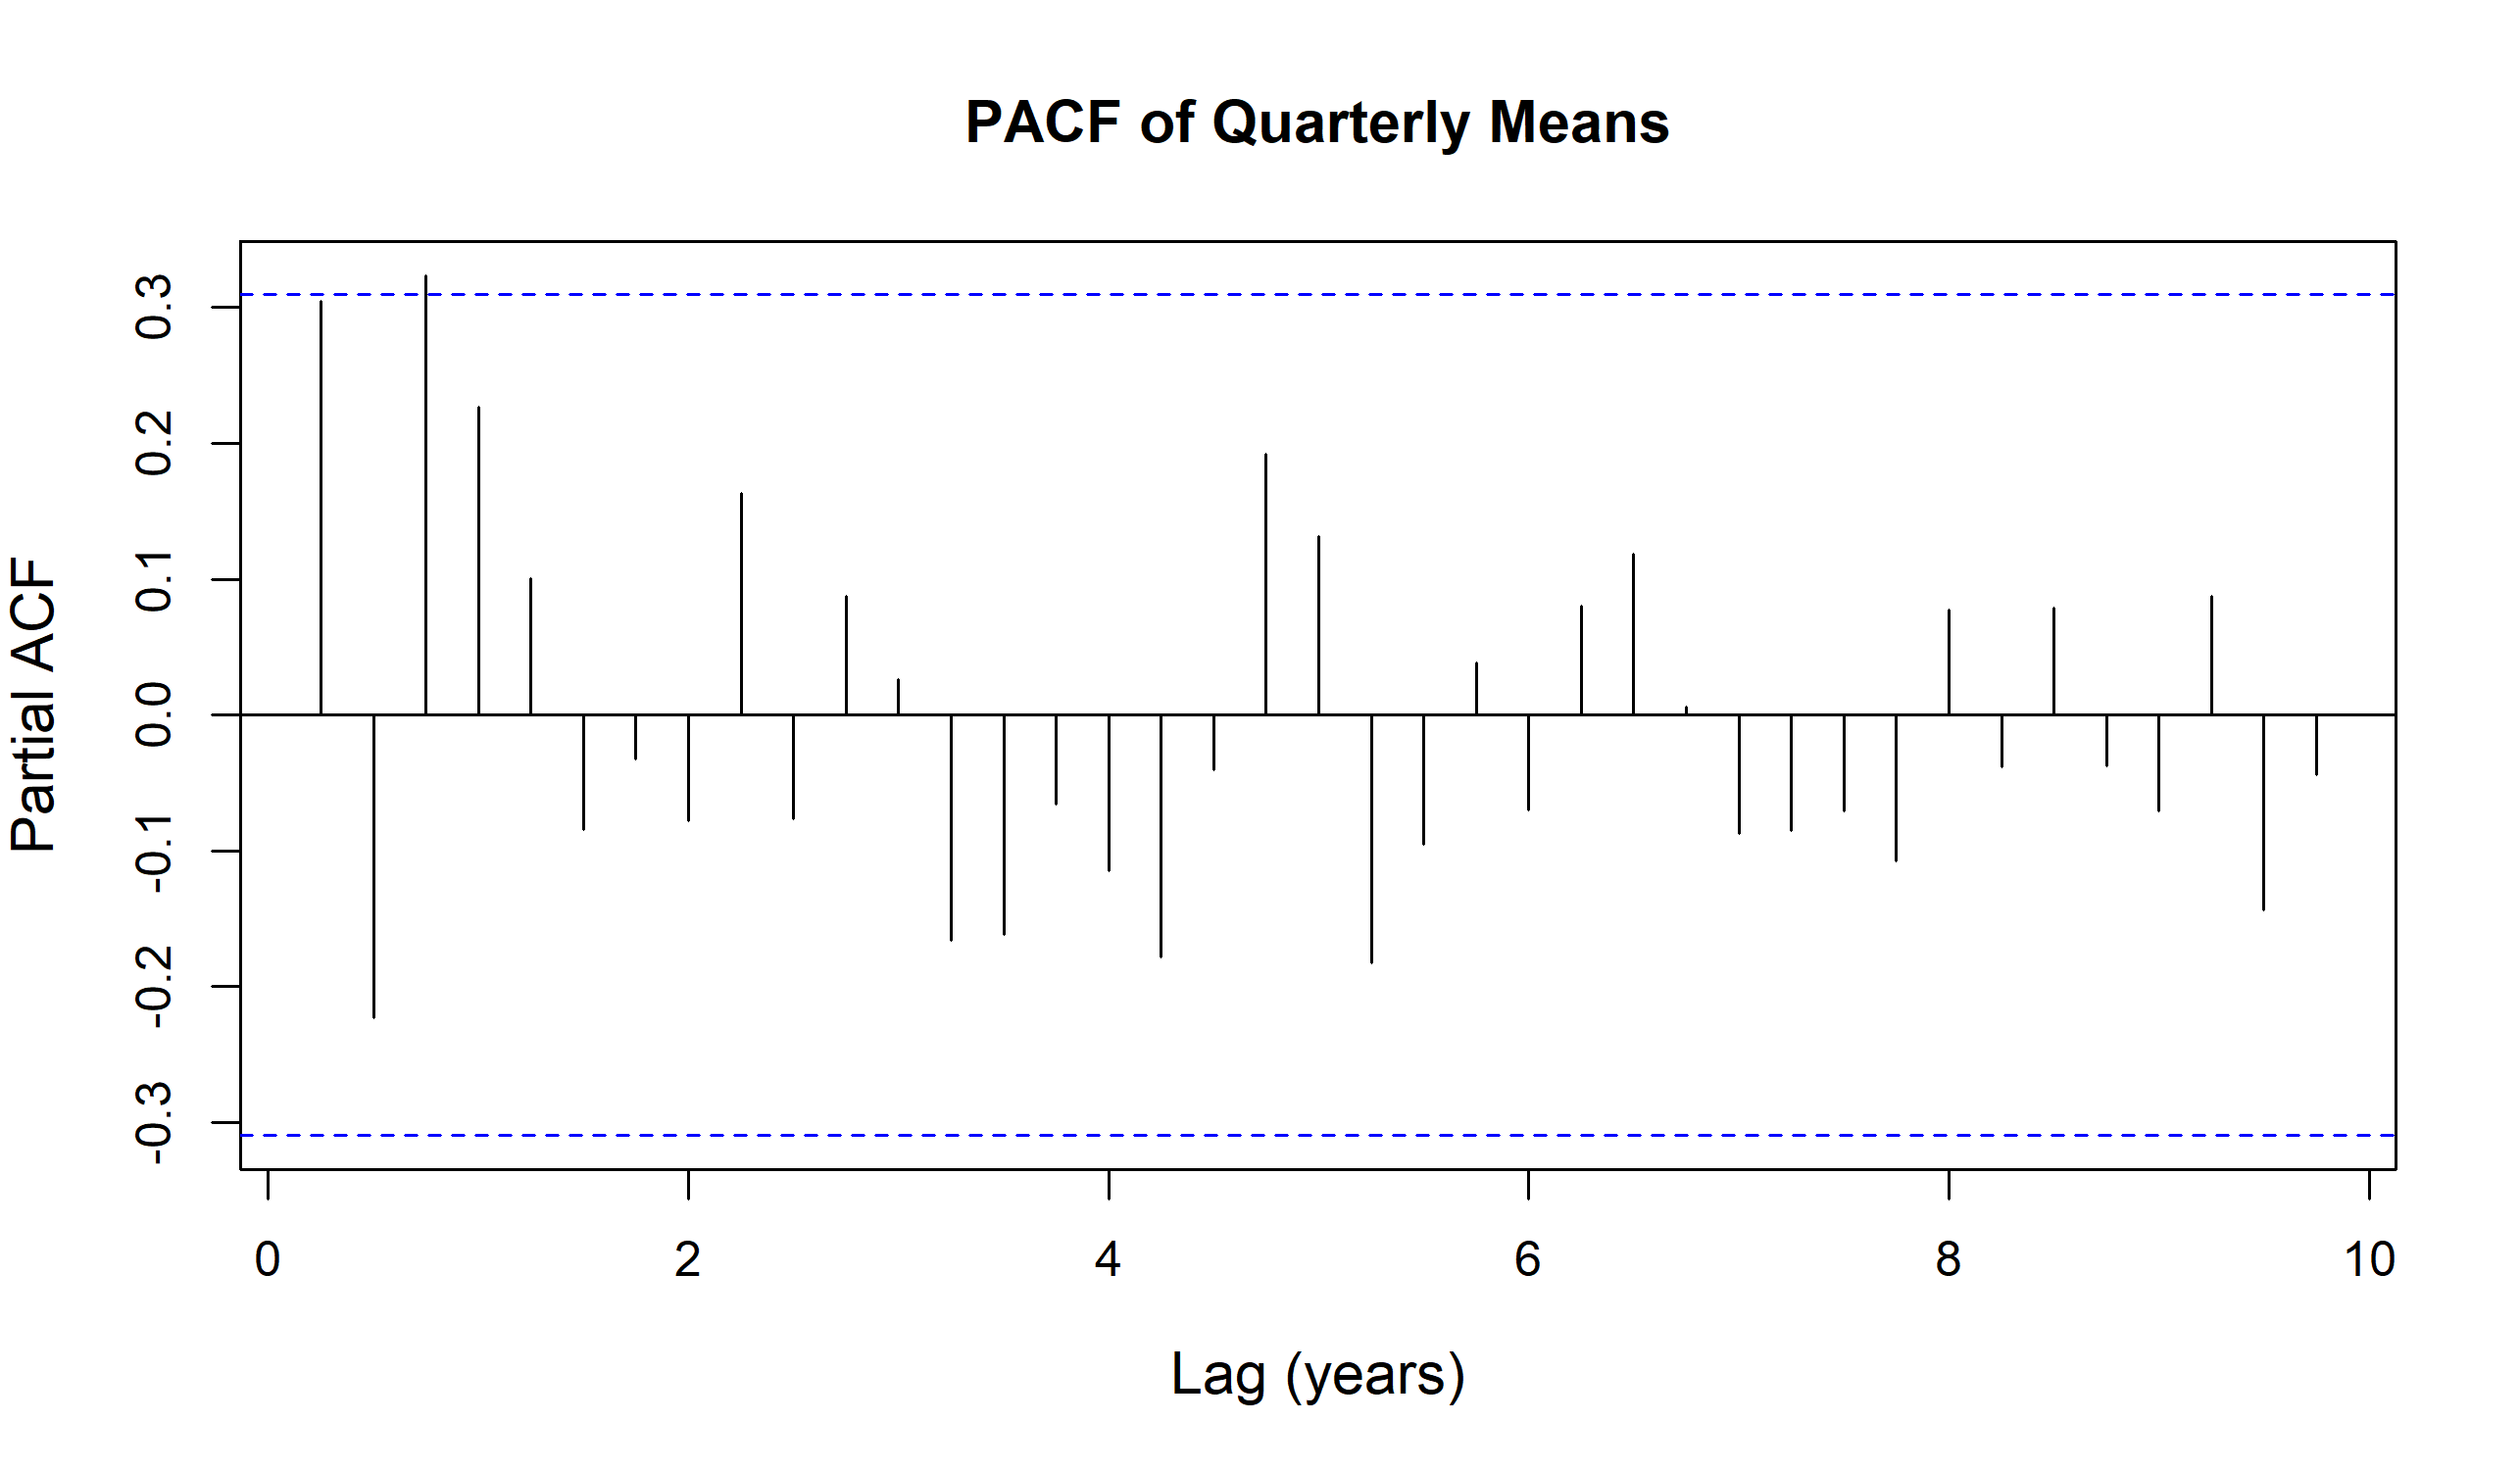
\includegraphics[width=\textwidth]{Sections/ARIMA/Plots/PACF.png}
        \subcaption{Partial auto correlation function}\label{S2fig:PACF}
    \end{subfigure}
\caption{Auto correlation and partial auto correlation functions of our quarterly means data plotted for different lag values in years, with 95\% significance level shown in blue.}
\label{S2fig:ACFPACF}
\end{figure}

We will fit several ARMA models for varying values, $(p,q) \in [0,3]\times[0,7]$ and calculate both the AIC and BIC of the fit. This produces the following results:

\begin{table}[H]
    \begin{center}
        \csvautotabular{S2Tab1.csv}
    \end{center}
    \caption{Sum of AIC and BIC for different $(p,q)$ pairs. For $q > 7$ or $p > 3$ the parameter pair approach the end of the stationarity region.}
    \label{S2:tab_sum}
\end{table}

\begin{itemize}
    \item \input{Sections/ARIMA/Outputs/min1.txt}
    \item \input{Sections/ARIMA/Outputs/min2.txt}
    \item \input{Sections/ARIMA/Outputs/min3.txt}
\end{itemize}

It is worth mentioning that the models allowed for there to be a mean and the best fit was calculated by first using conditional-sum-of-squares to find starting values, then maximum likelihood.
\nline
Continuing with $p = 0$ and $q=1$, we shall take the residuals of our $\ARMA{0}{1}$ model and plot them against time along with there ACF and the distribution of the residuals. This can be seen in \autoref{S2fig:manual_res}. It seems we have removed the correlation between points from looking at the ACF, performing a Ljung-Box test returned a p-value of \input{Sections/ARIMA/Outputs/manual_res.txt}. This indicates the residuals are independent \cite{10.1093/biomet/65.2.297}. However, we can also see that the residuals do not fit well to a normal distribution. It is for this reason we will try other parameters.

\begin{figure}[H]
    \centering
    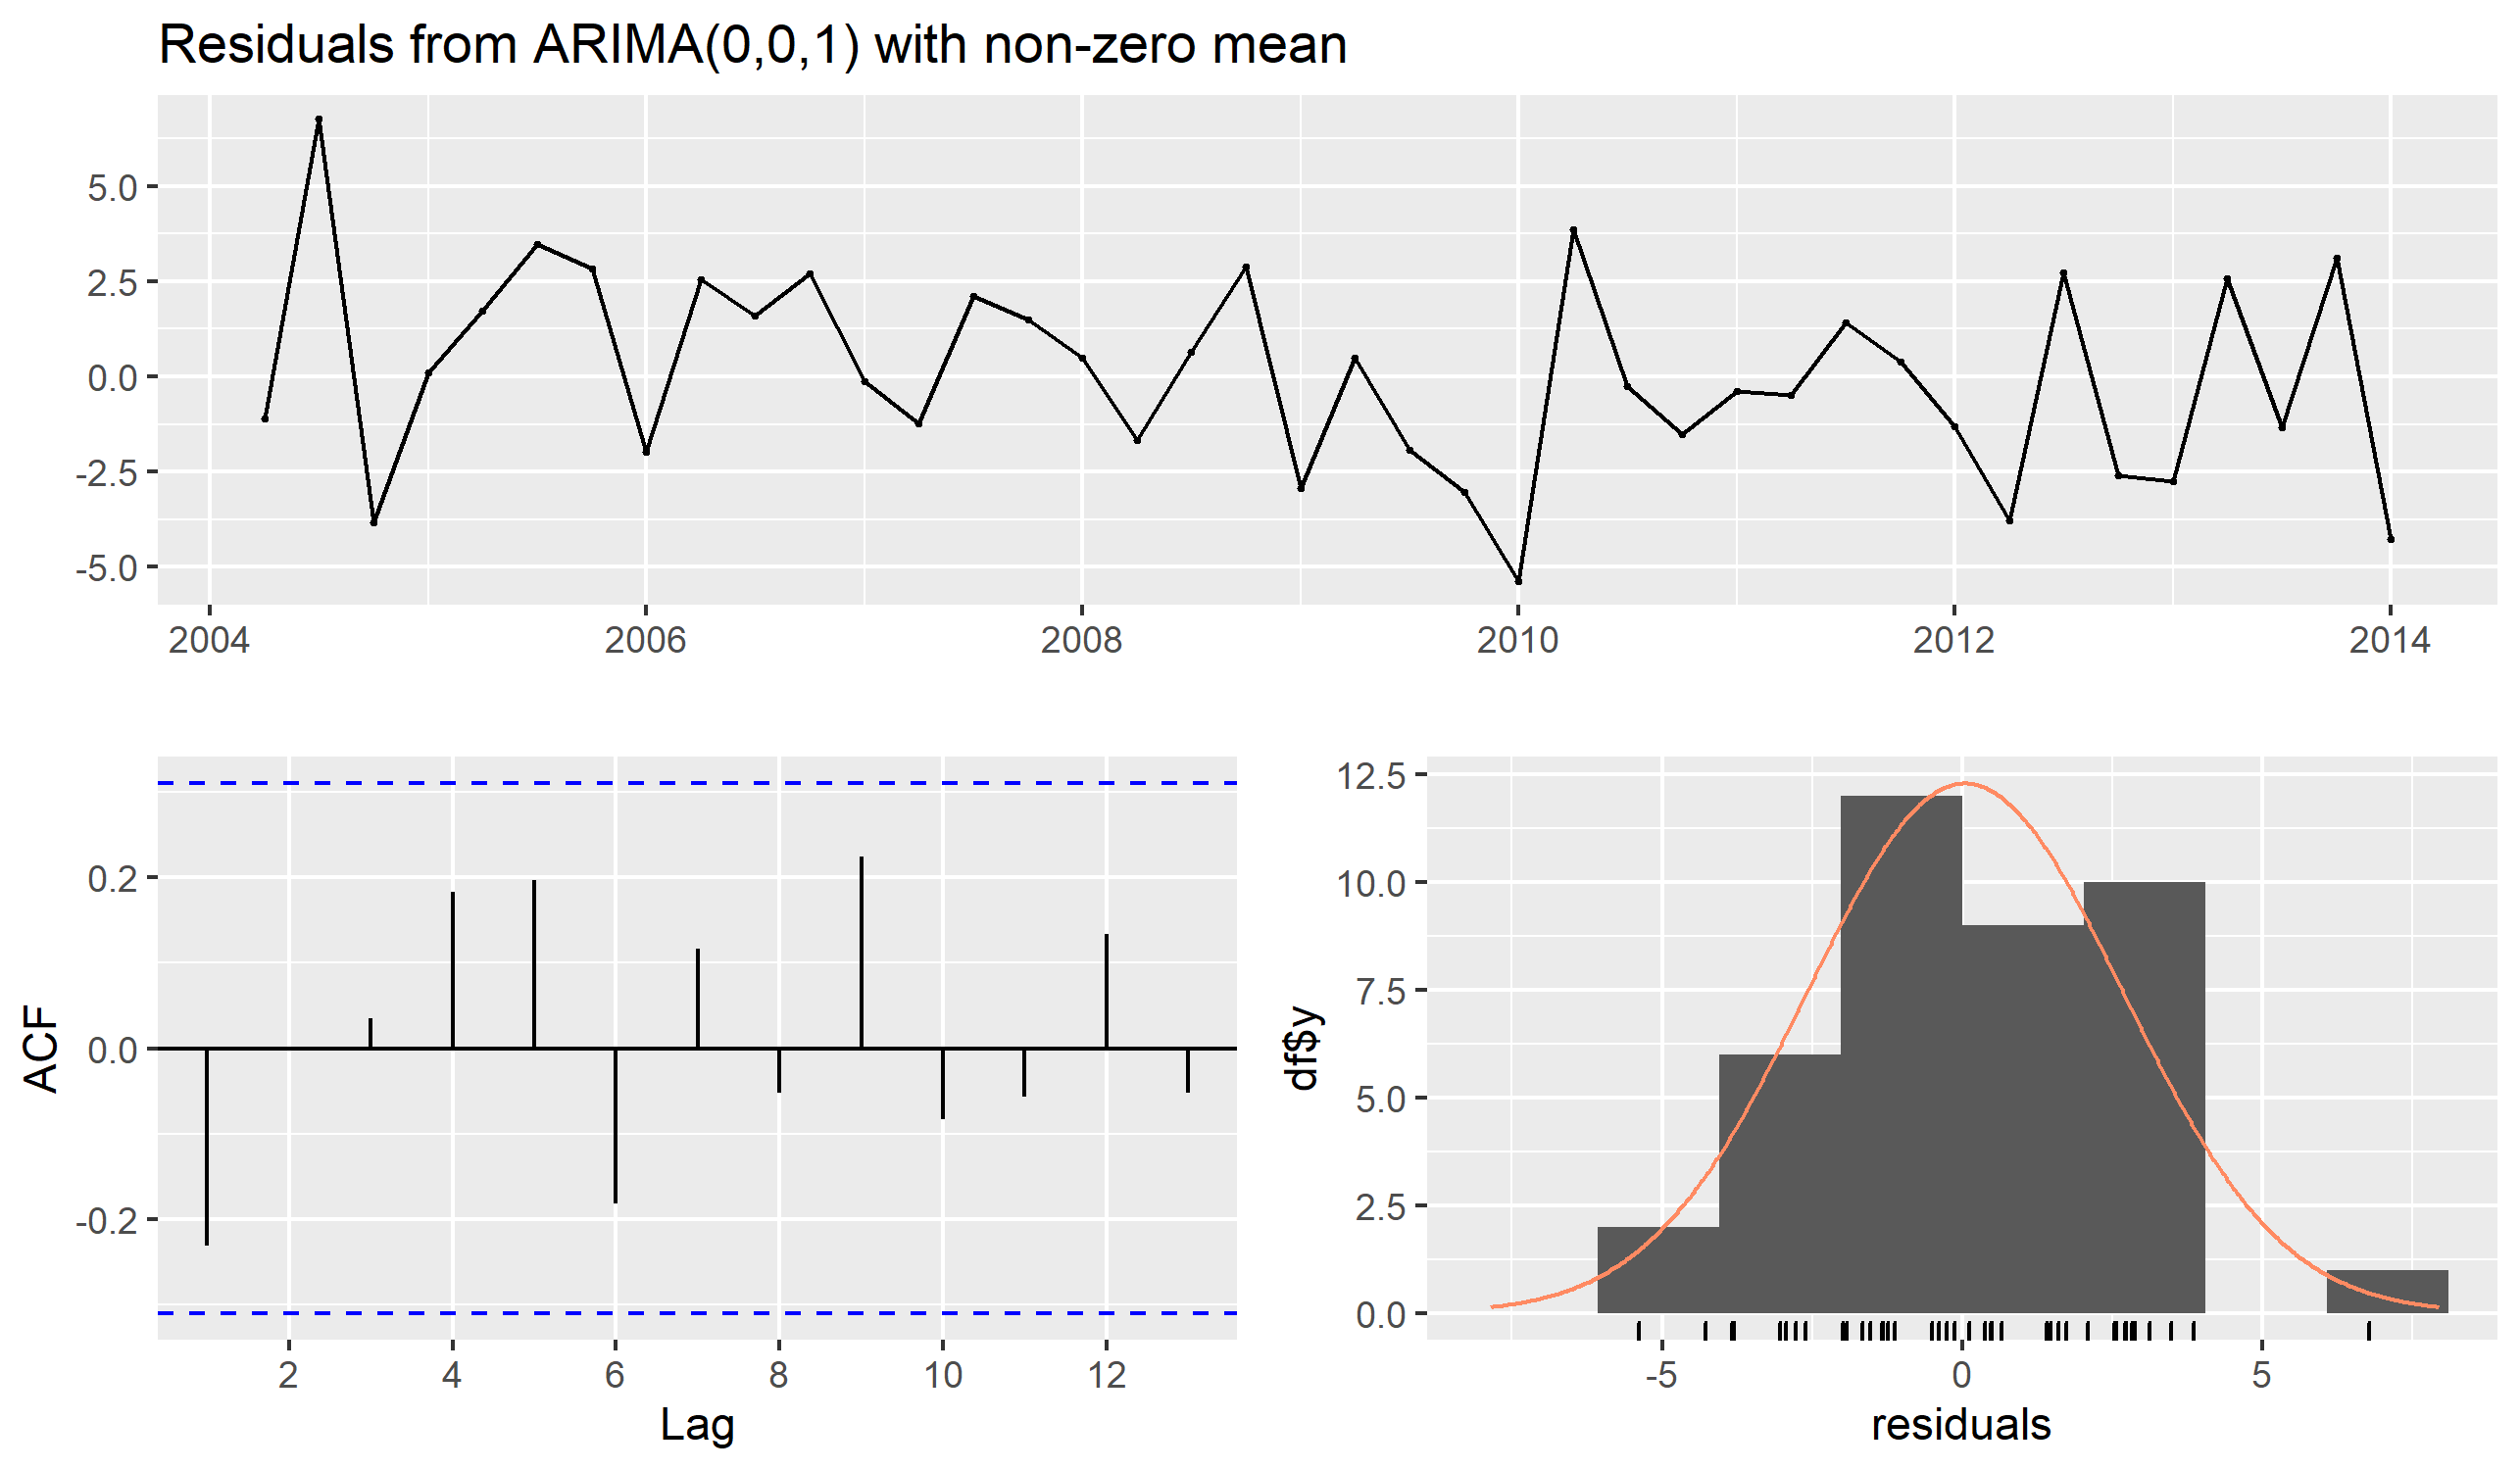
\includegraphics[width=\sTwoRes\textwidth]{Sections/ARIMA/Plots/manual_res.png}
    \caption{Residuals from our $\ARMA{0}{1}$ model plotted against time. The ACF between residuals and their distribution.}
    \label{S2fig:manual_res}
\end{figure}

In an attempt to find parameters which fit better we refer to the "auto.arima()" function which is from the R package "forecast" \cite{forecast}. This is a function which uses a variation of the Hyndman-Khandakar algorithm \cite{hyndman2008automatic}, which combines unit root tests, minimisation of the AICc (Second-order Akaike Information Criterion) and MLE to obtain an ARIMA model.
\nline
When using AICc as the measure of so-called "goodness" we are told that $p=0$ and $q=2$ are optimal. The residuals of our $\ARMA{0}{2}$ model can be seen in \autoref{S2fig:auto_res}. We can immediately see that the residuals follow the normal distribution much better. Also, we still have low correlation between points from looking at our ACF. Performing a Ljung-Box test we get a p-value of \input{Sections/ARIMA/Outputs/auto_res.txt}, this again indicates independence between our residuals.

\begin{figure}[H]
    \centering
    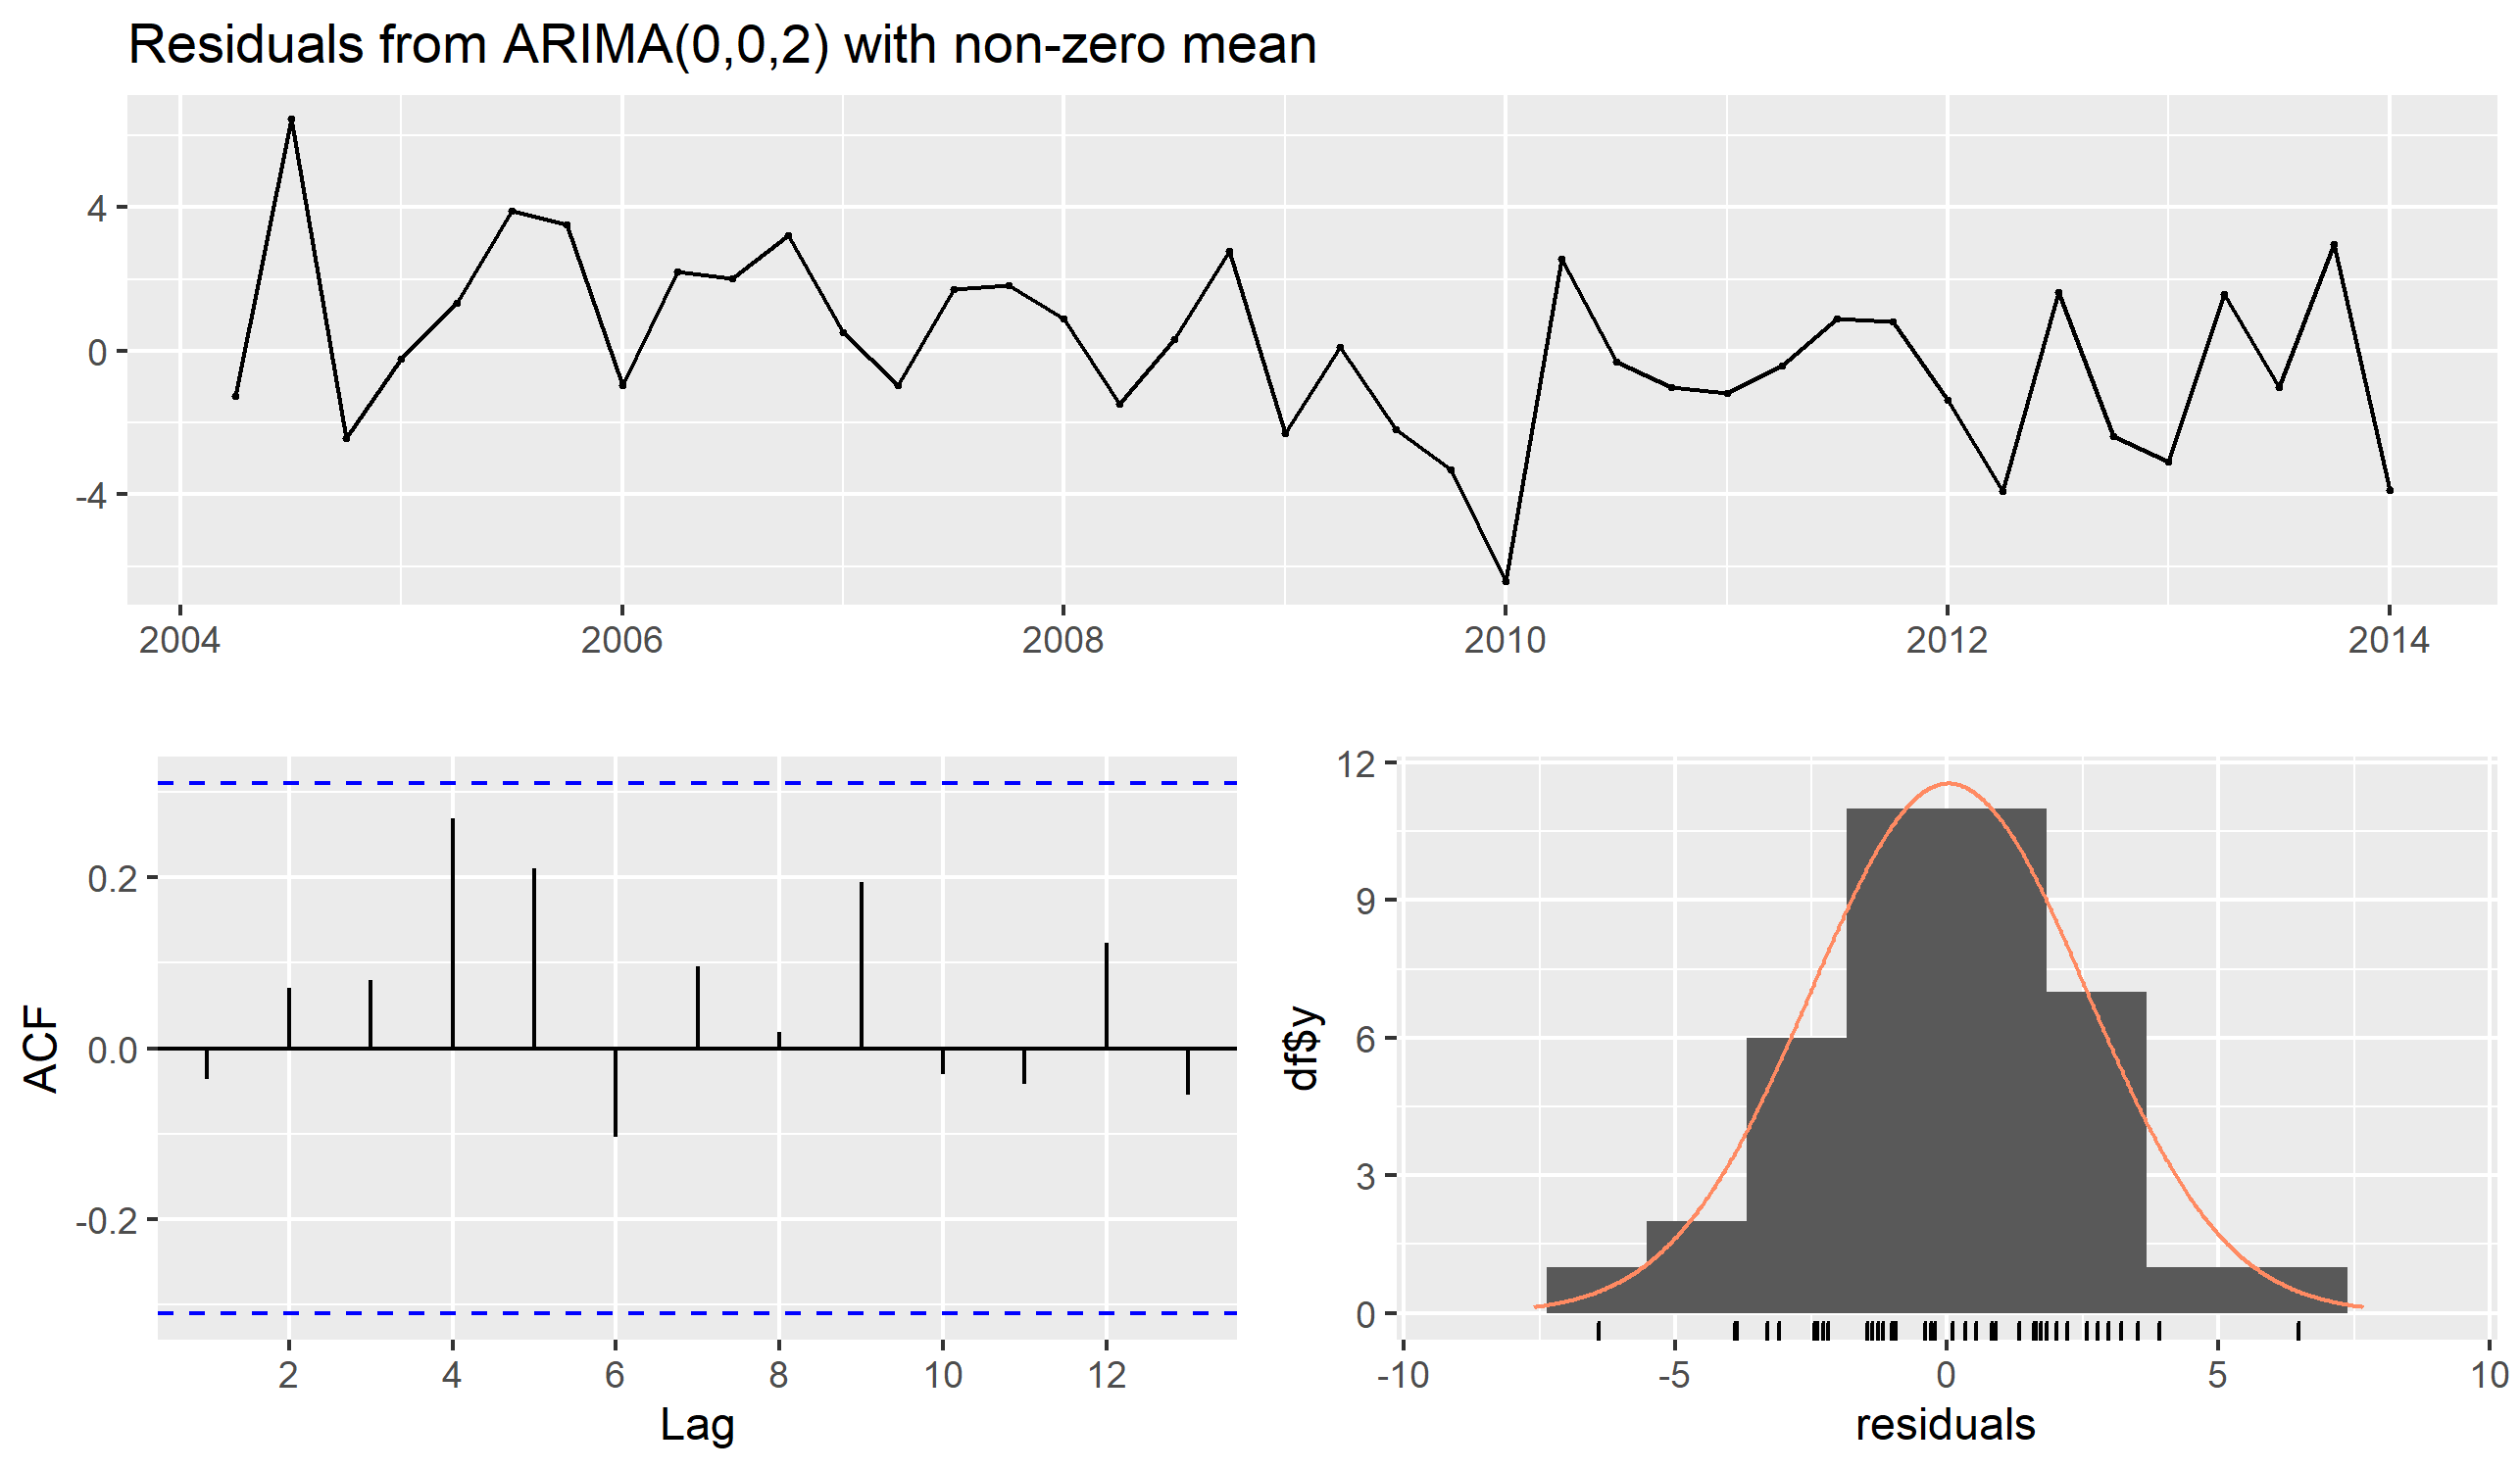
\includegraphics[width=\sTwoRes\textwidth]{Sections/ARIMA/Plots/auto_res.png}
    \caption{Residuals from our $\ARMA{0}{2}$ model plotted against time. The ACF between residuals and their distribution.}
    \label{S2fig:auto_res}
\end{figure}

\subsubsection{Building our model}

Accepting $p=0$ and $q=2$ as our optimal parameters, from our maximum likelihood (MLE) method our full model is:

\begin{equation*}
    x_t = 16.87 + 0.63\epsilon_{t-1} - 0.24\epsilon_{t-2} \quad \epsilon_t \sim \text{N}\left(0, 6.835\right)
\end{equation*}
\nline
Now, using this model to forecast 6 quarters ahead of our data.

\begin{figure}[H]
    \centering
    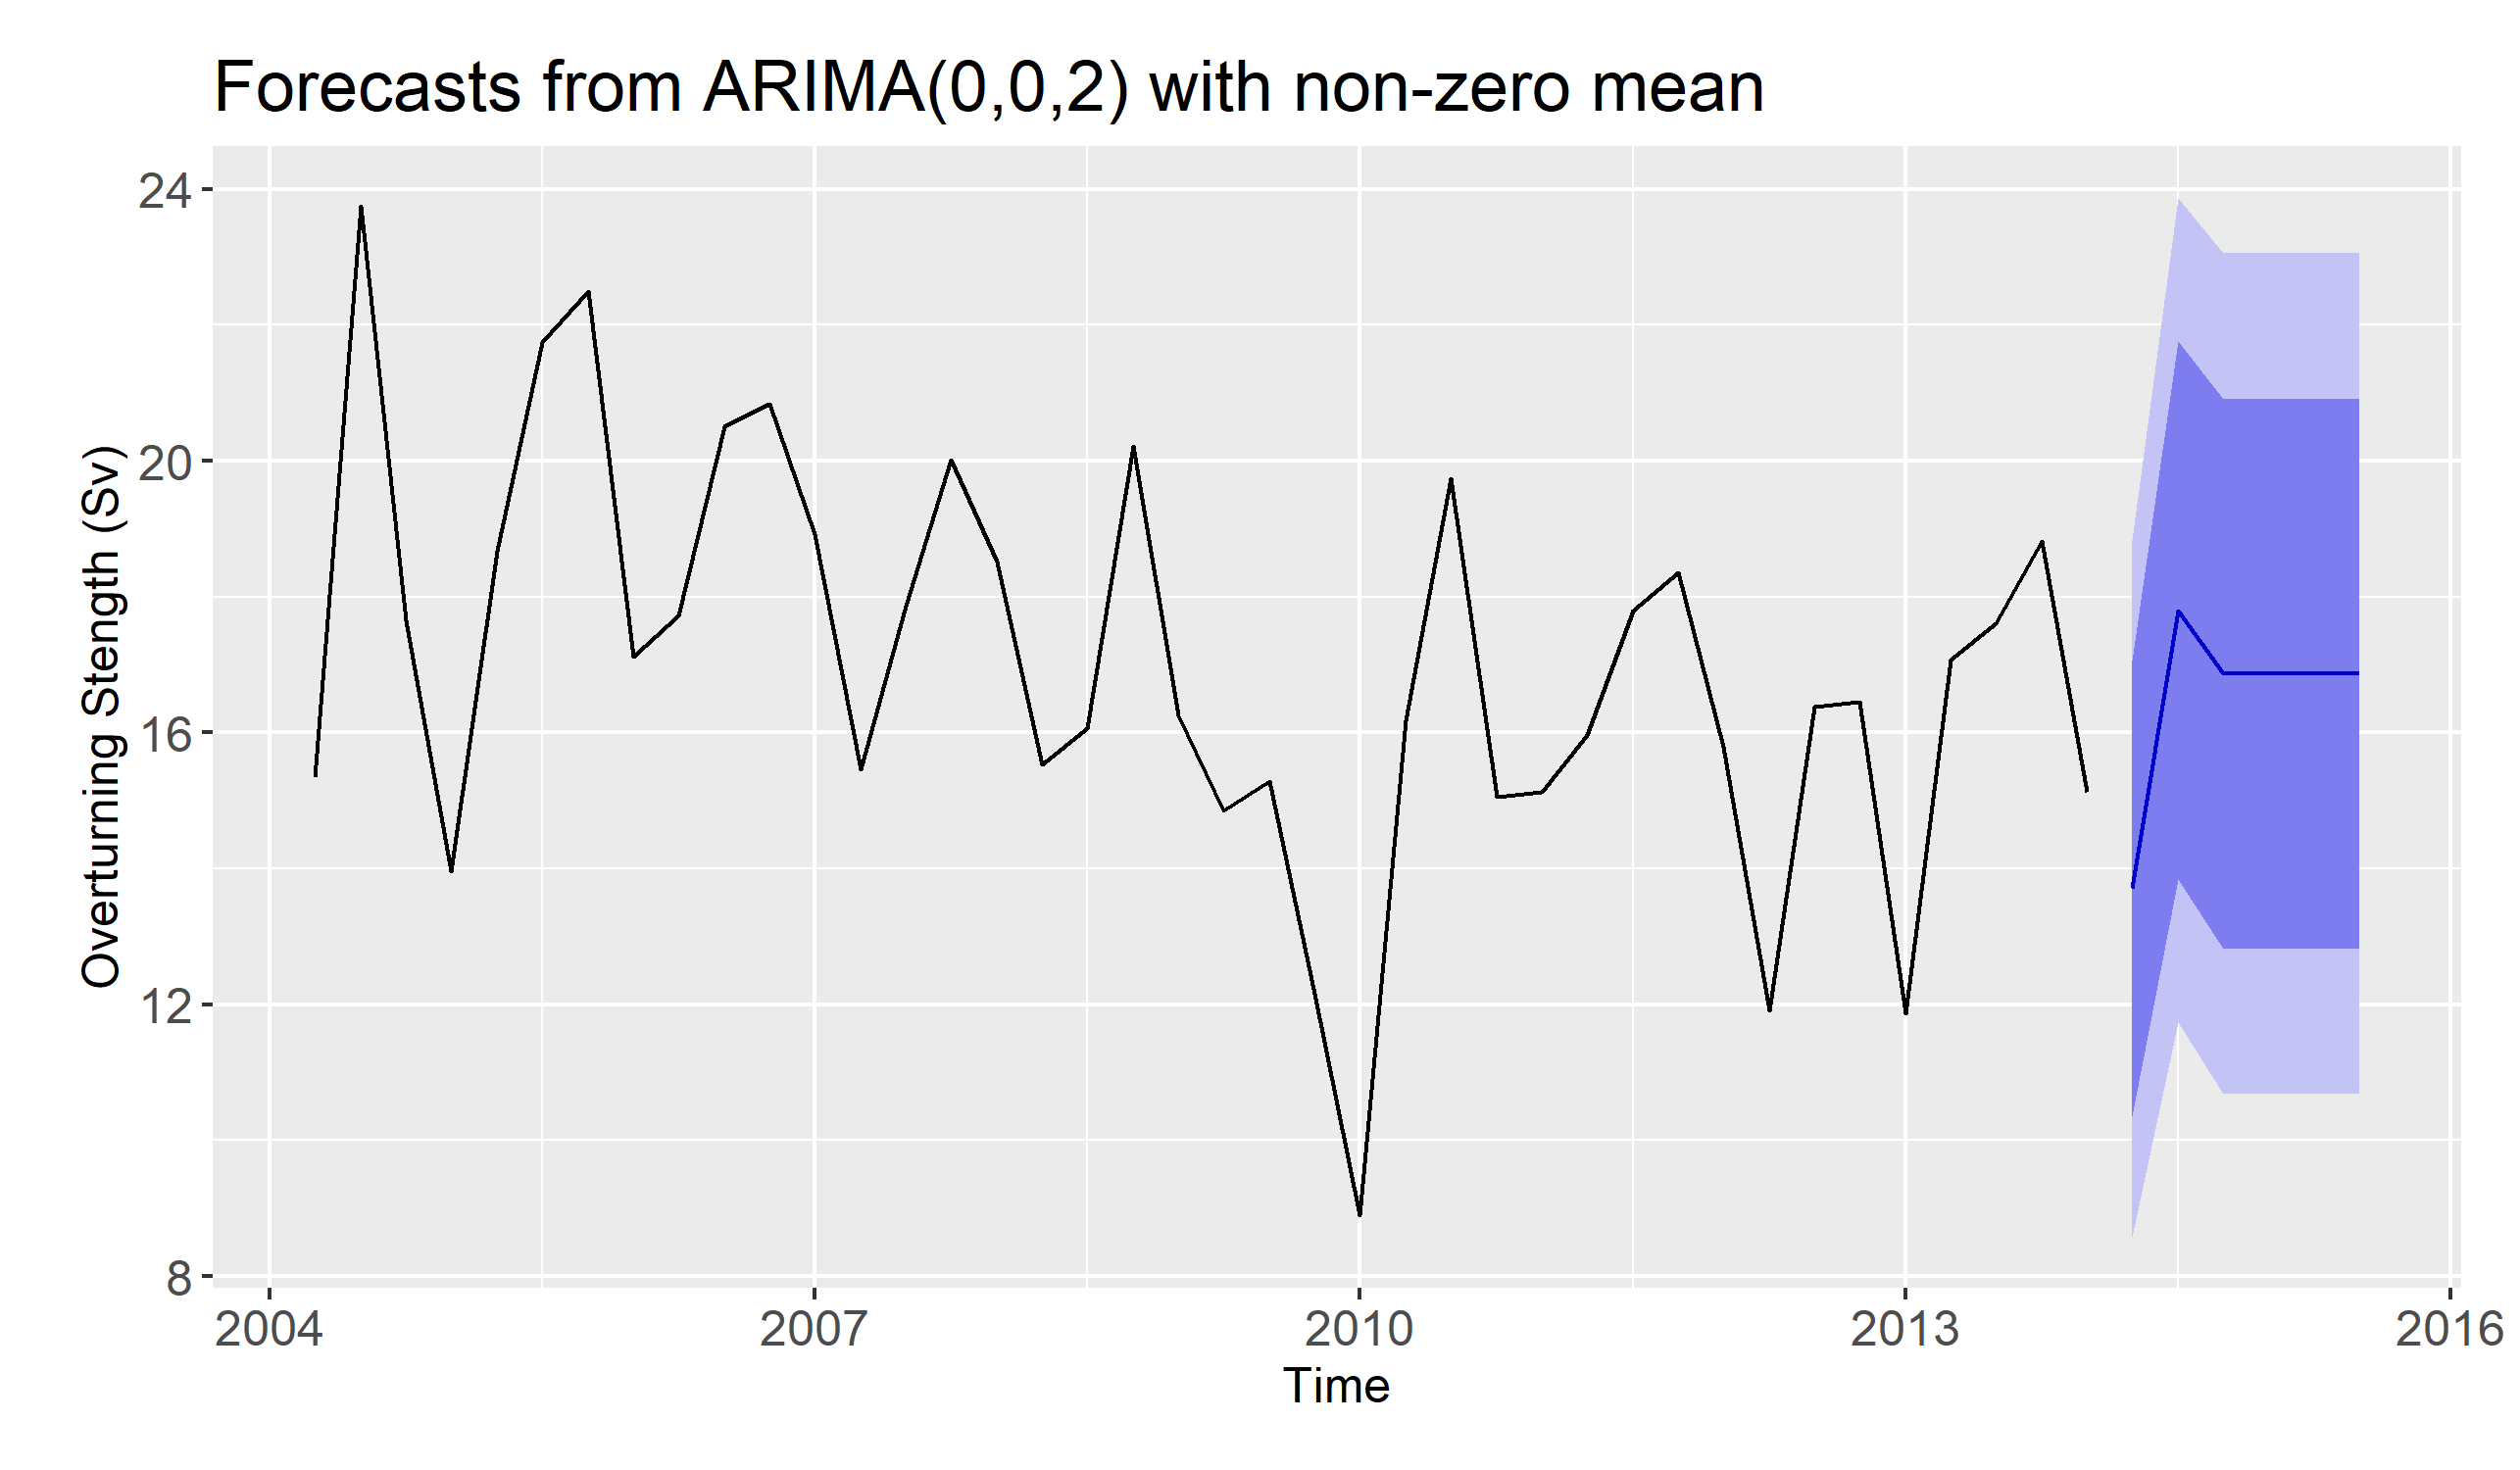
\includegraphics[width=0.50\textwidth]{Sections/ARIMA/Plots/forecast.png}
    \caption{Forecast of overturning strength (Sv) 6 quarters into the future with 80\% and 95\% confidence intervals shown in dark blue and light blue respectively.}
    \label{S2fig:ARMA forecast}
\end{figure}

?Discussion?

\subsection{Autoregressive Integrated Moving Average Model (ARIMA)}

An ARIMA model consists of three parameters, $p$, $q$ and $d$. $p$ and $q$ are identical to an ARIMA model and $d$ is the degree of differencing (the number of times the data have had past values subtracted). 

\subsubsection{Finding optimal parameters}

To find the optimal parameters we will again use the "auto.arima" function mentioned in \autoref{SSec:fop1}.
\nline
The optimal parameters determined are $p=0$, $d=1$ and $q=0$. Checking the residuals of our $\ARIMA{0}{1}{0}$ model as we did previously:

\begin{figure}[H]
    \centering
    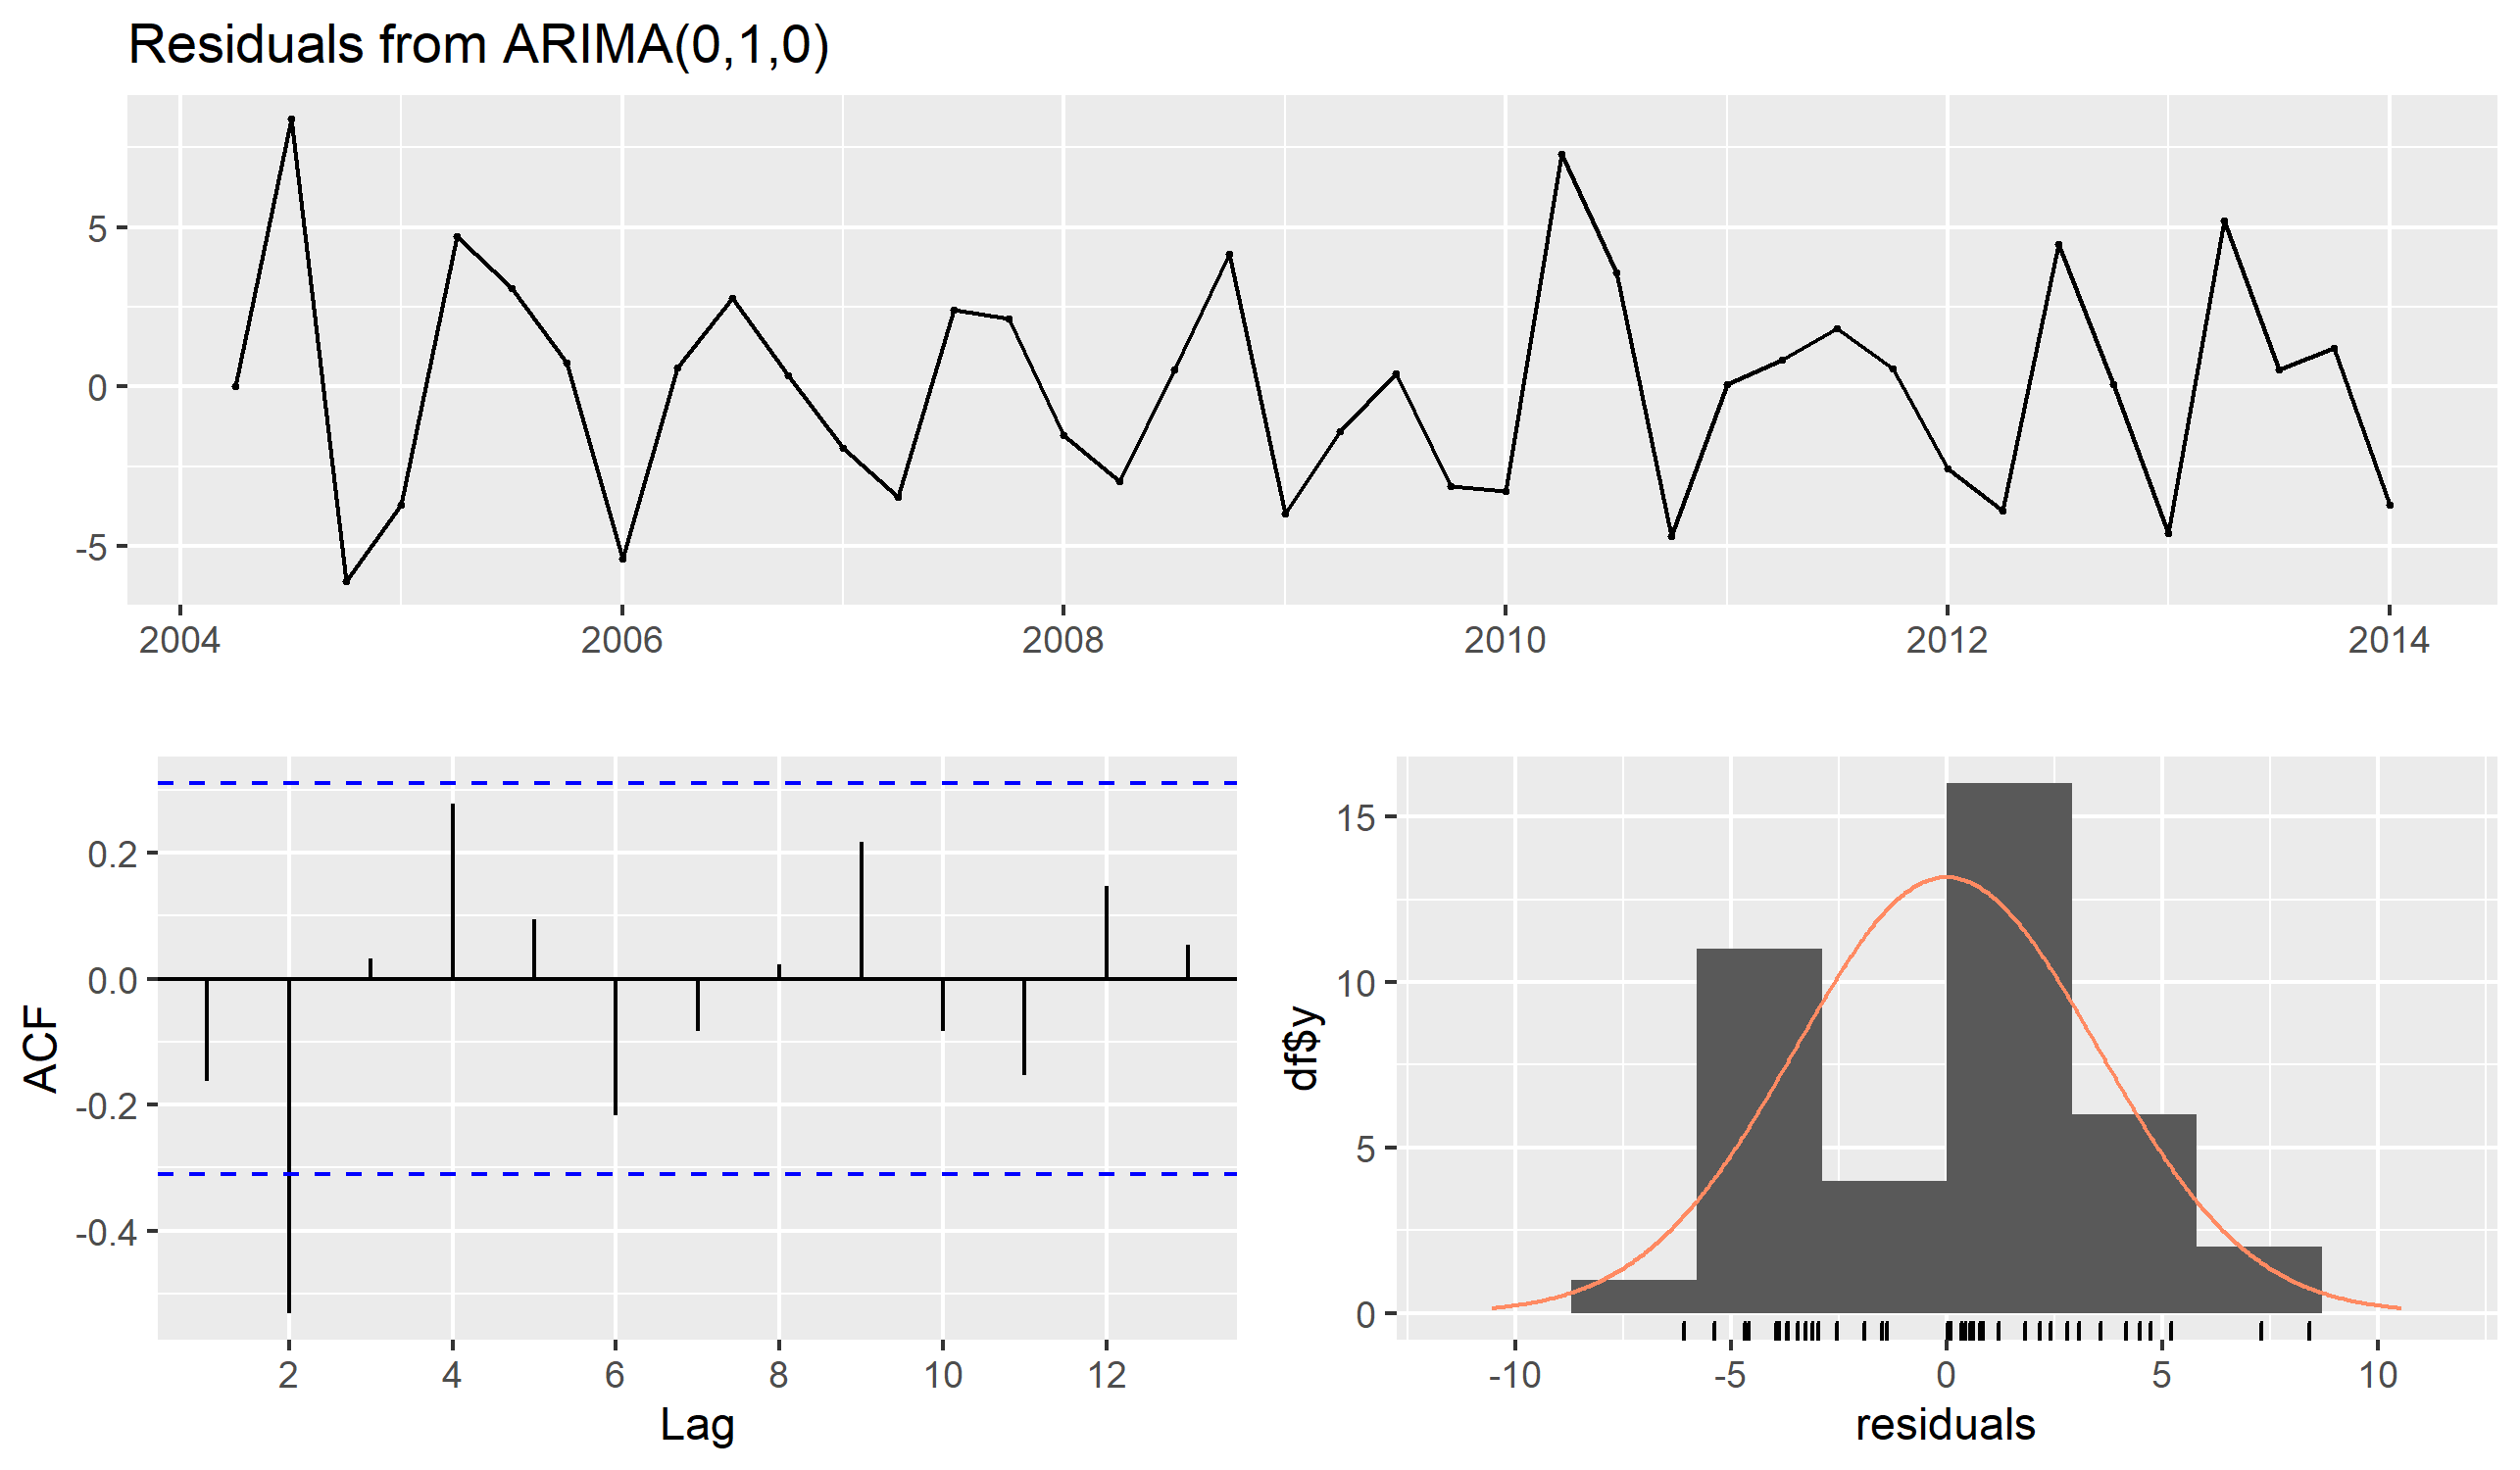
\includegraphics[width=\sTwoRes\textwidth]{Sections/ARIMA/Plots/auto__arima_res.png}
    \caption{Residuals from our $\ARIMA{0}{1}{0}$ model plotted against time. The ACF between residuals and their distribution.}
    \label{S2fig:arima_res}
\end{figure}

We can see from \autoref{S2fig:arima_res} that the distribution does not appear to be normal and from the ACF plot we can see that there appears to be some correlation between the residuals; this is confirmed by a p-value of 0.01 from our Ljung-Box test. This p-value indicates that the data are not independently distributed; they exhibit serial correlation \cite{10.1093/biomet/65.2.297}.
\nline
After experimenting with forcing different $d$ values into the "auto.arima" function, a better parameter triplet was found: $\ARIMA{4}{2}{0}$

\begin{figure}[H]
    \centering
    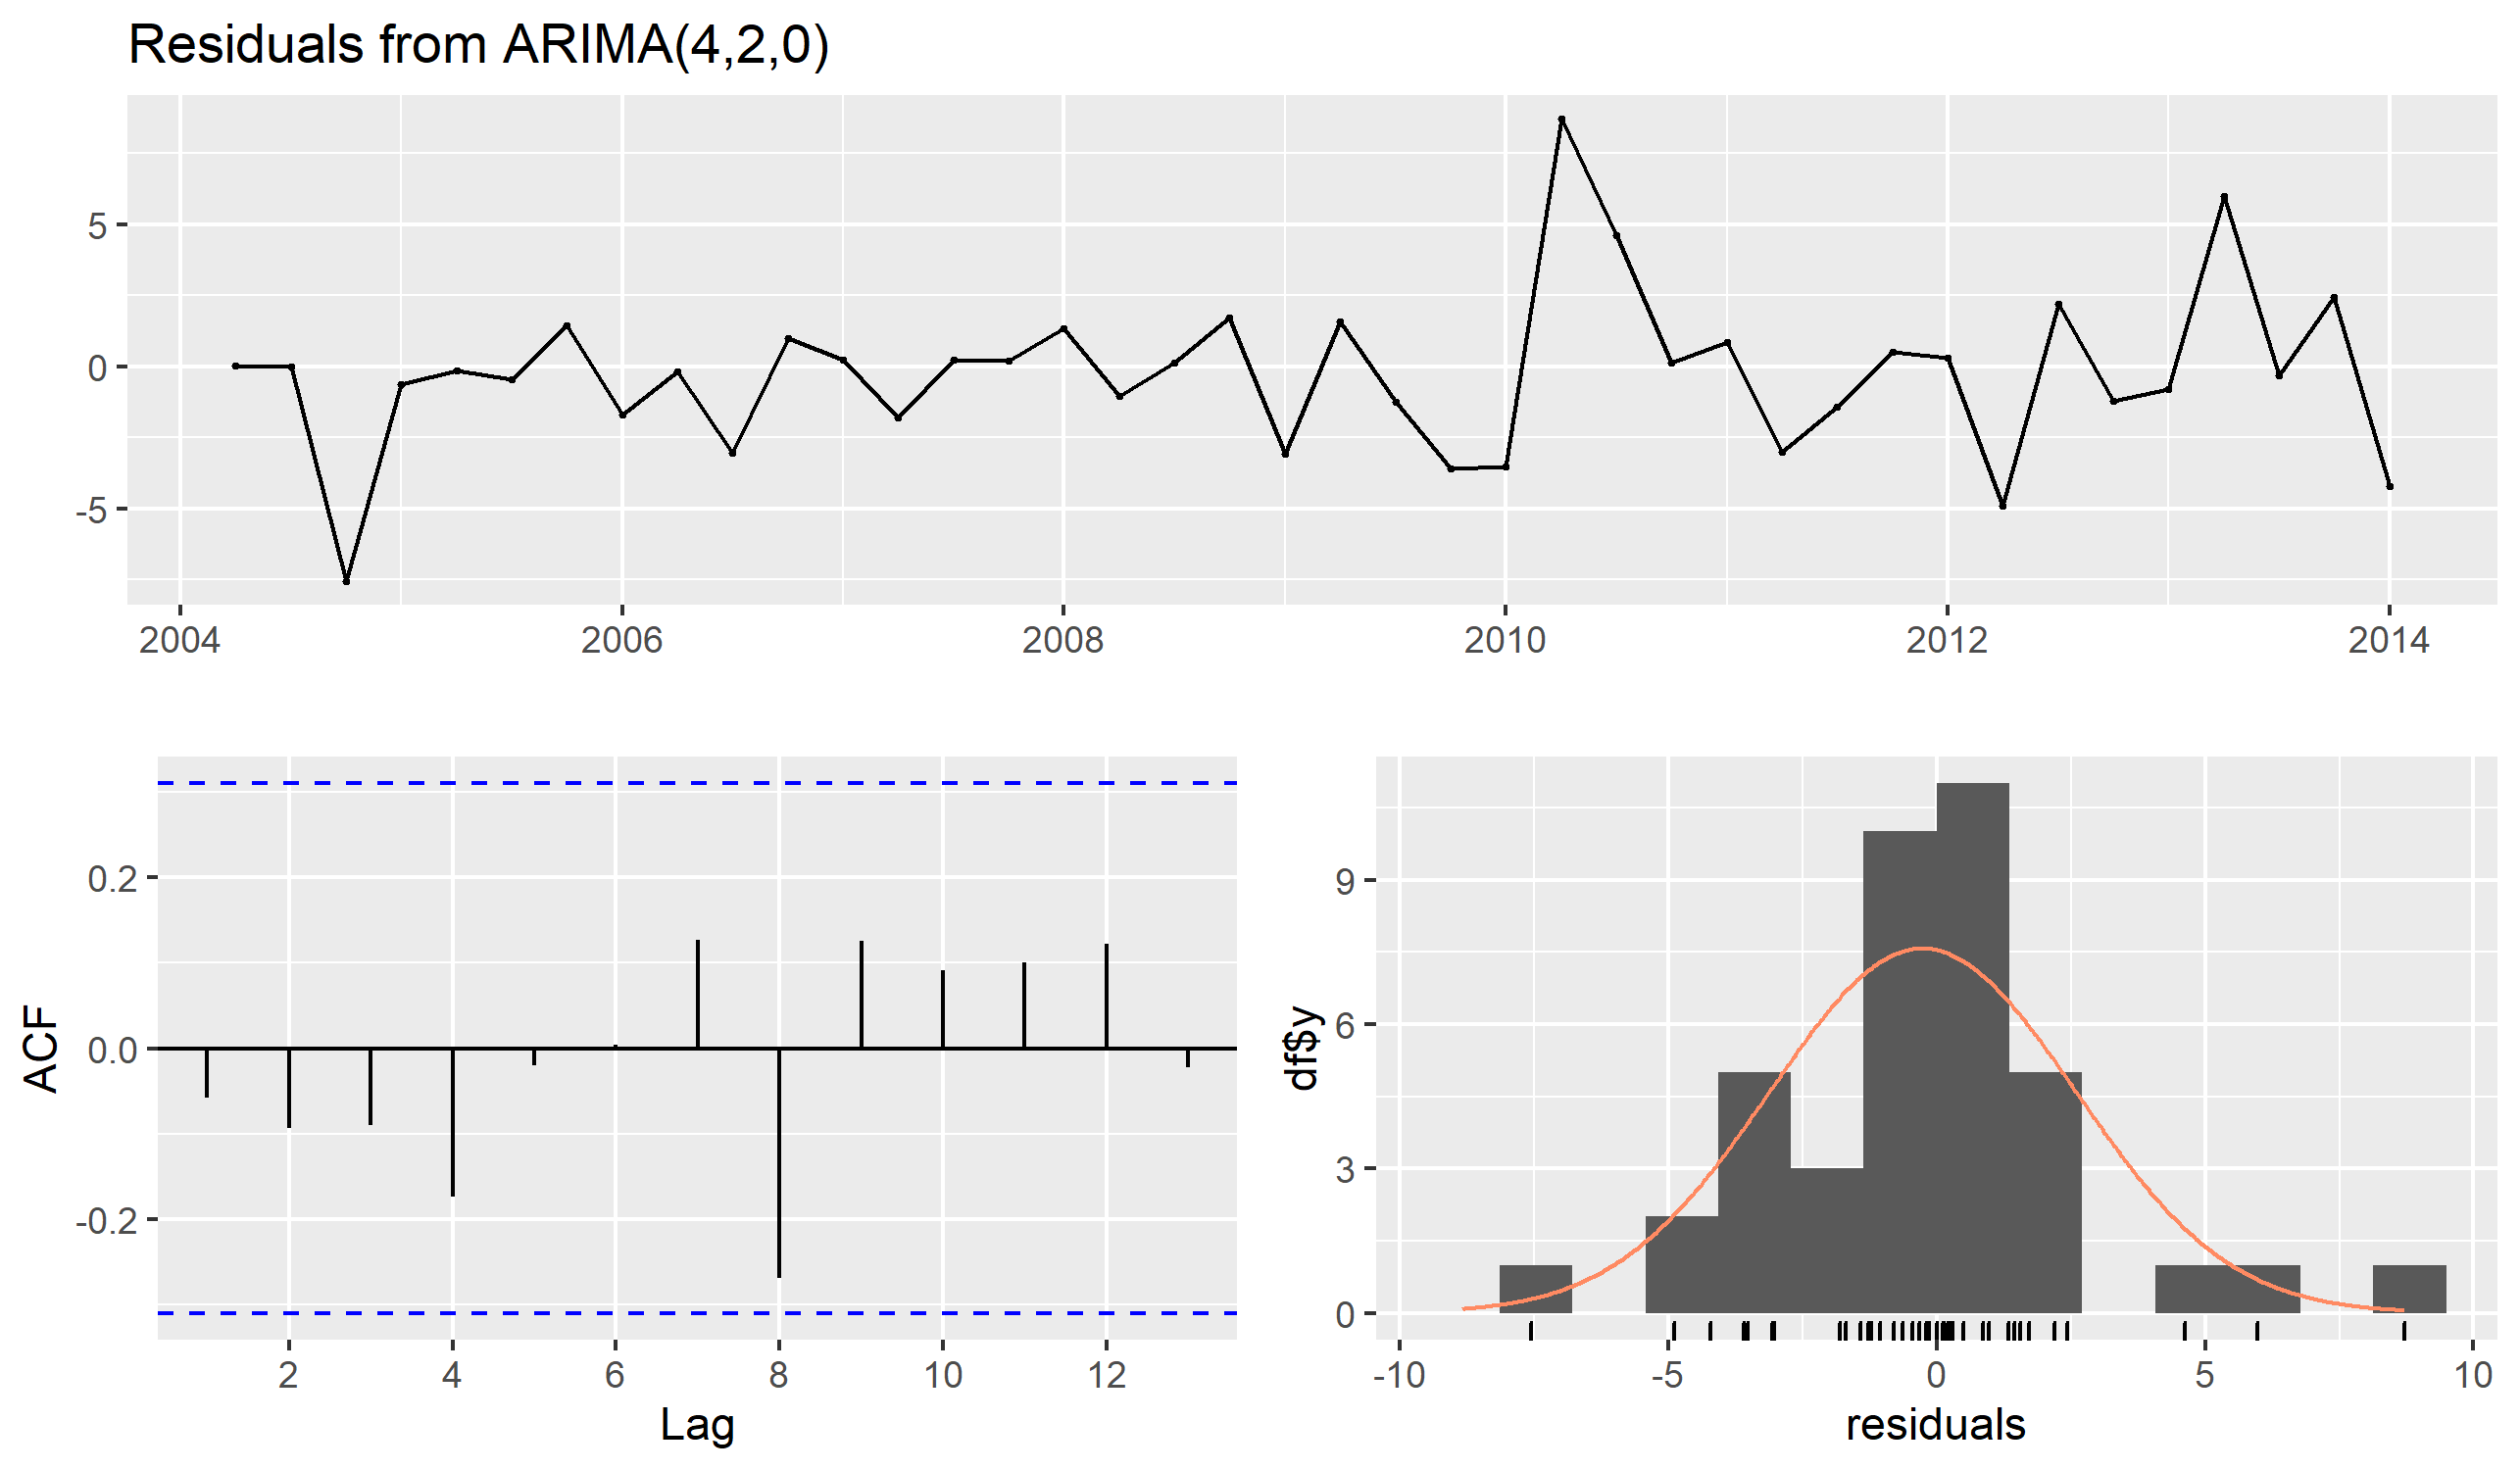
\includegraphics[width=\sTwoRes\textwidth]{Sections/ARIMA/Plots/auto__arima_res2.png}
    \caption{Residuals from our $\ARIMA{4}{2}{0}$ model plotted against time. The ACF between residuals and their distribution.}
    \label{S2fig:arima_res2}
\end{figure}

We can see in \autoref{S2fig:arima_res2} that we have managed to remove the correlation between residuals in the ACF and our p-value from our Ljung-Box test is \input{Sections/ARIMA/Outputs/auto_arima_res2.txt} which indicates independence. However, we can see that our distribution of residuals are not normal.


\subsubsection{Building our model}

Our $\ARIMA{4}{2}{0}$ model has the following coefficients:

\begin{lstlisting}[caption={ARIMA(4,2,0) Coefficients}]
Coefficients:
          ar1      ar2      ar3      ar4
      -1.0195  -1.3529  -0.9128  -0.5612
s.e.   0.1473   0.1666   0.1627   0.1527
\end{lstlisting}

Now, forecasting 6 quarters ahead with our model:

\begin{figure}[H]
    \centering
    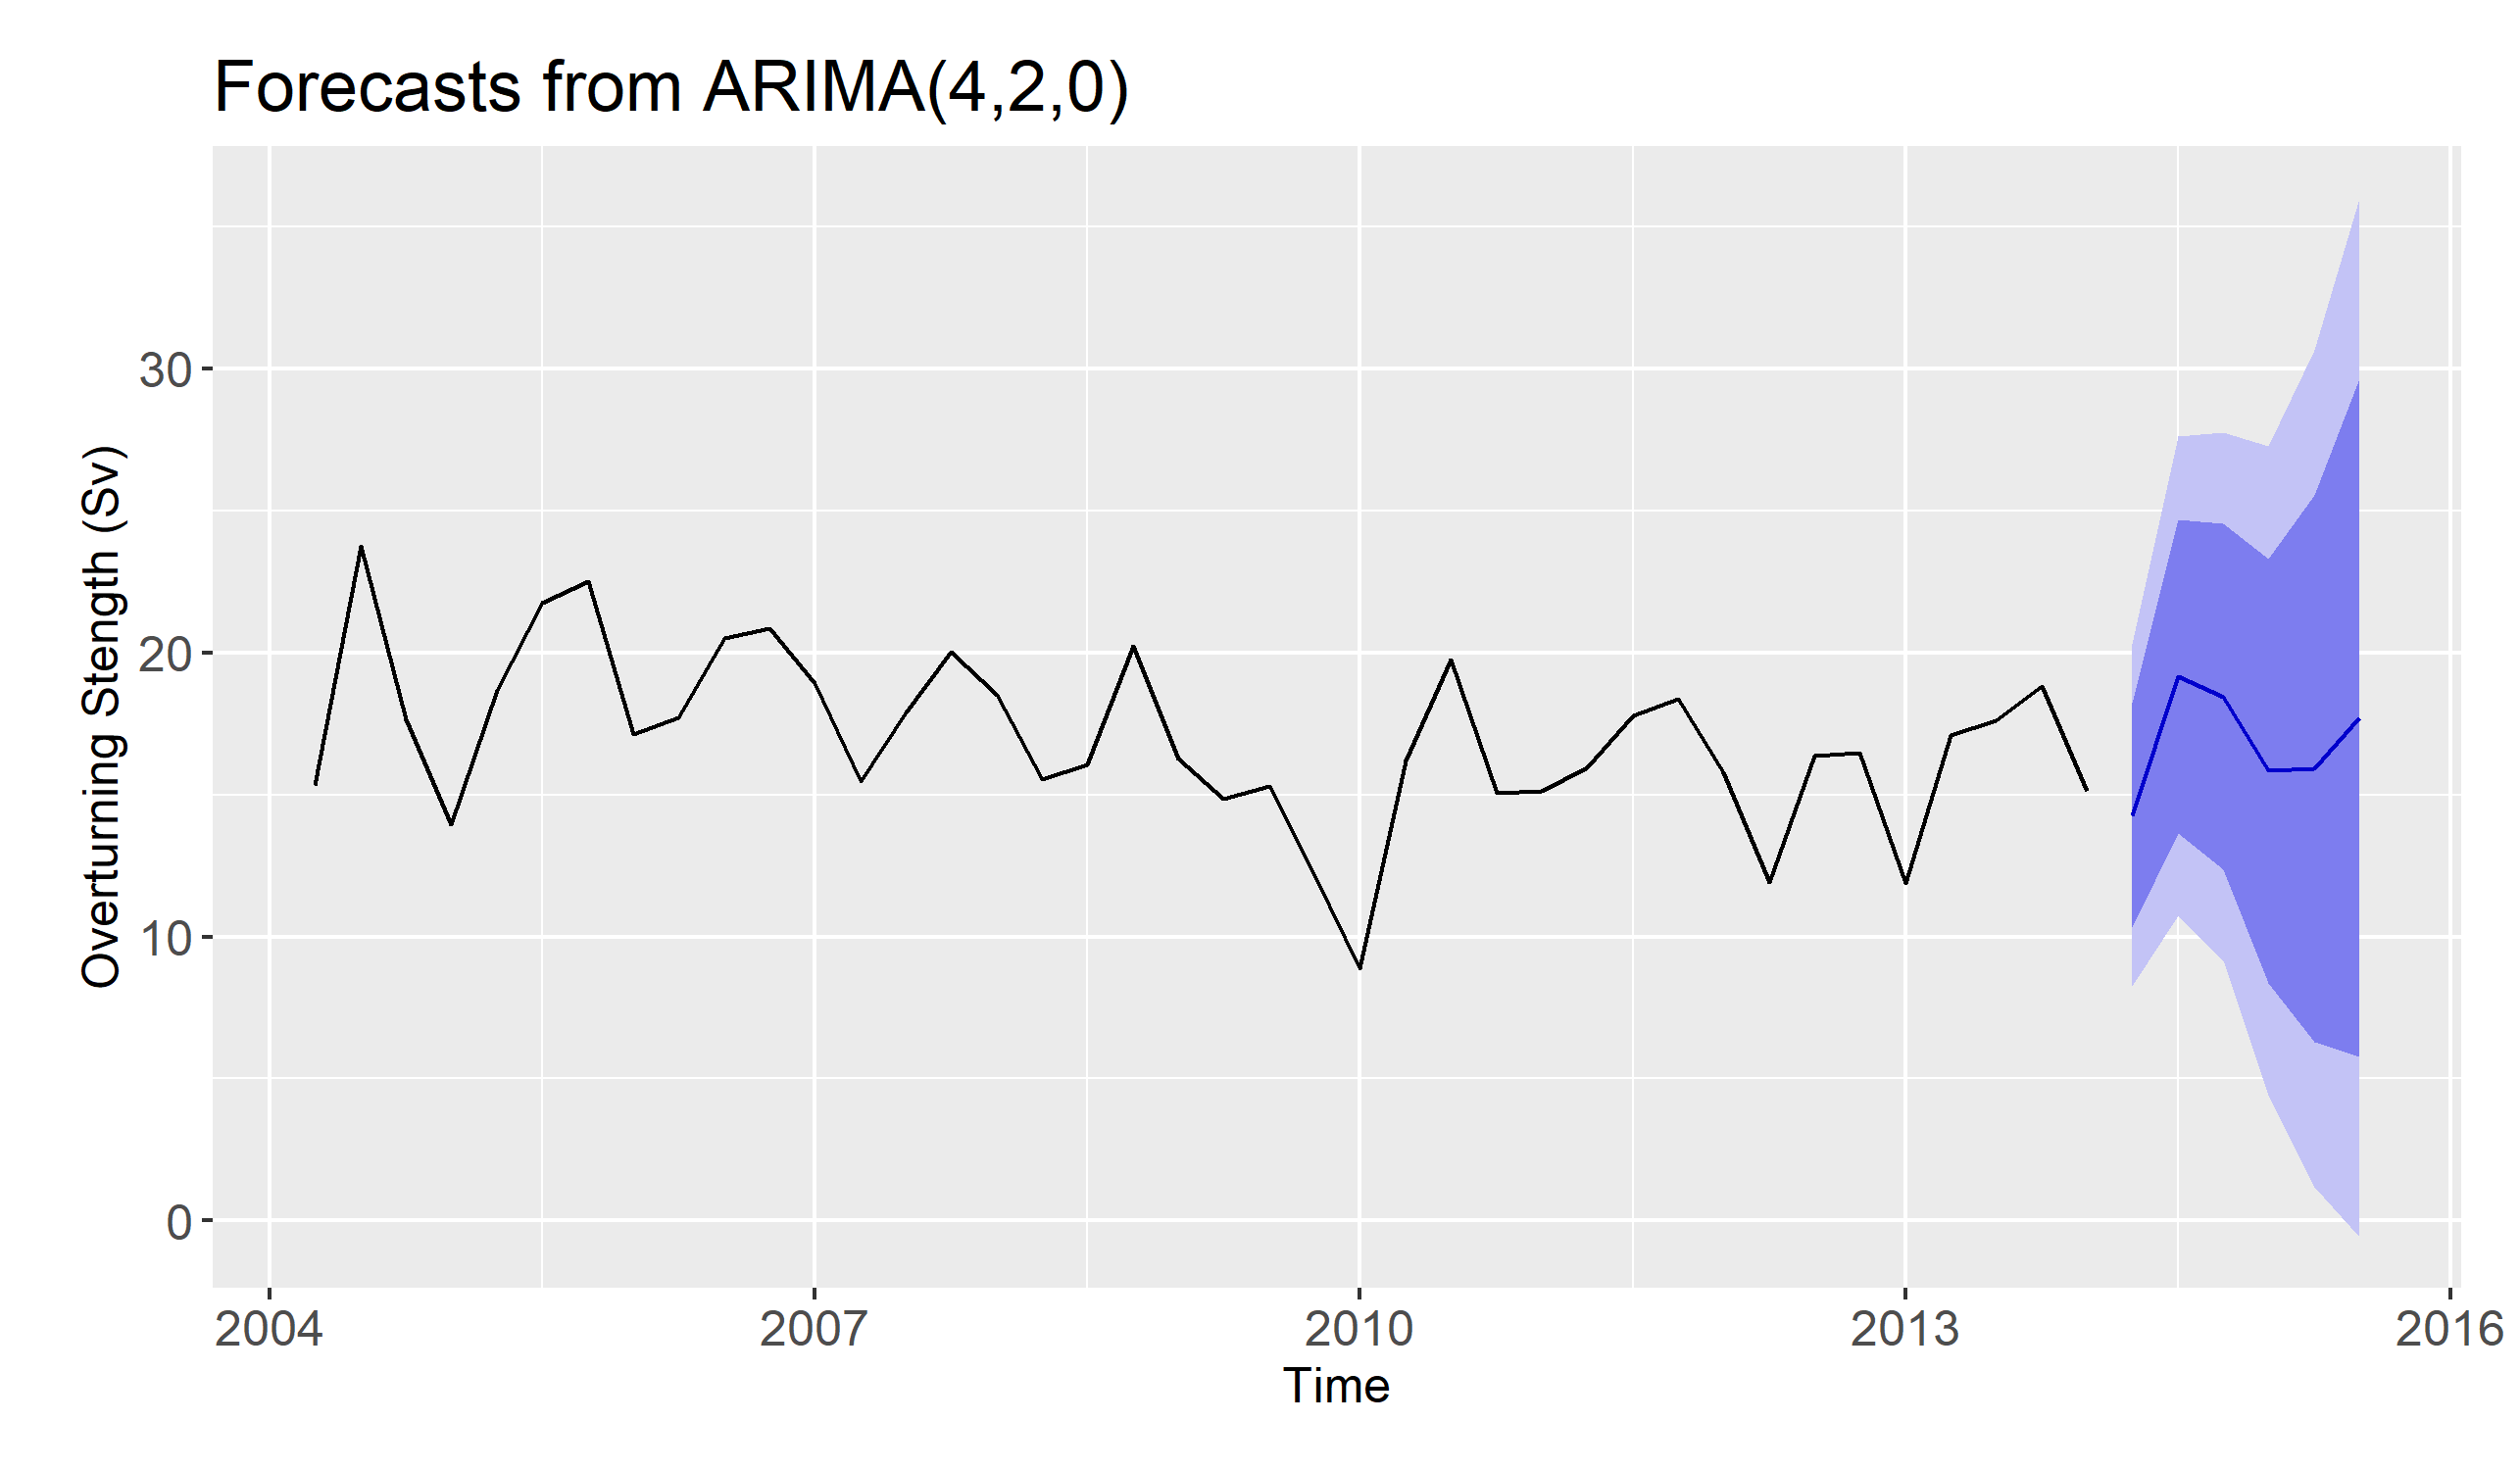
\includegraphics[width=0.50\textwidth]{Sections/ARIMA/Plots/forecast_arima.png}
    \caption{Forecast of overturning strength (Sv) 6 quarters into the future with 80\% and 95\% confidence intervals shown in dark blue and light blue respectively.}
    \label{S2fig:Arima_Forecast}
\end{figure}
\pagebreak
\subsection{Comparing our ARMA and ARIMA Models}

Here is quick overview of each model:

\begin{lstlisting}[caption={ARMA(0,2)}]
    ARIMA(0,0,2) with non-zero mean

    Coefficients:
             ma1      ma2     mean
          0.6323  -0.2403  16.8684
    s.e.  0.1461   0.1367   0.5528
    
    sigma^2 = 6.835:  log likelihood = -94.29
    AIC=196.57   AICc=197.72   BIC=203.33
    \end{lstlisting}

\begin{lstlisting}[caption={ARIMA(4,2,0)}]
    ARIMA(4,2,0)

    Coefficients:
              ar1      ar2      ar3      ar4
          -1.0195  -1.3529  -0.9128  -0.5612
    s.e.   0.1473   0.1666   0.1627   0.1527
    
    sigma^2 = 9.443:  log likelihood = -96.26
    AIC=202.51   AICc=204.39   BIC=210.7
    \end{lstlisting}

    We can see that the ARMA model has the best fit for all 4 measurements (log likelihood, AIC, BIC and AICc). This is reflected in the forecast made by the models where the ARMA model has much smaller confidence intervals. However, the forecast for the ARIMA model seems to take on a shape that closer resembles the previous behavior in the time series, opposed to the ARMA models near straight line.